\documentclass{polytech/polytech}
\usepackage{tikz}

%-----------Configuration du rapport-----------------

\schooldepartment{peip}
\typereport{peip2}
\reportyear{2016-2017}
\title{DI 6 Correcteur de posture assise à base d'Arduino}
\reportlogo{image/logo_1ere_couverture} %A changer avec la photo de 1ere de couverture
\student{Jérémy}{LOCHE}{jeremy.loche@etu.univ-tours.fr}
\student{Dimitrios}{KOKKONIS}{dimitrios.kokkonis@etu.univ-tours.fr}
\academicsupervisor[di]{Sébastien}{BEAUFILS}{sebastien.beaufils@univ-tours.fr}

%------------Poster------------------

\posterblock{Titre 1 poster}{texte 1 poster}{image/poster_1}{légende 1 poster}

\posterblock{Titre 2 poster}{texte 2 poster}{image/poster_1}{légende 2 poster}

\posterblock{Titre 3 poster}{texte 3 poster}{image/poster_1}{légende 3 poster}




%------------------Résumés & mots clés------------

\resume{Ce projet a pour but de créer un correcteur de posture assise d'une personne, sous la forme d'un système embarqué. Le projet est basé sur un Arduino Uno, qui gère les données de quatre capteurs de charges placées sous les pieds d'une chaise. On l'utilise ensuite pour transmettre ces données en série (soit par Bluetooth, soit par USB) à une application fonctionnant sur un ordinateur Windows/OSX/Linux ou un appareil Android. Cette application permet de visualiser la chaise, la position du barycentre de l'utilisateur dans une zone de confort calibrée par l'utilisateur.  On peut ainsi détecter si la posture de l'utilisateur est bonne; l'application l'informe visuellement quand ce n'est pas le cas. Le logiciel utilisé est écrit en Java et en C.}



\abstract{This project aims to create an application for correcting one's sitting posture, using both software and hardware. The project was built upon an Arduino Uno that handles the data sent by four load sensors placed under the feet of a chair, and which in turn modifies and sends that data in serial form (either by Bluetooth or by USB) to an application that runs on a Windows/OSX/Linux computer or an Android device. That device then provides the user with a graphic representation of the chair, the barycenter of the user, as well as a "deadzone" which is calibrated by the user, and is used to detect wether the user's posture is incorrect or not; the application informs the user visually when he is not properly seated. The software is written in Java and C.}


\motcle{Correction de posture, Système embarqué, Arduino, Java, C}

\keyword{Posture correction, Embedded system, Arduino, Java, C}


\begin{document}

\chapter*{Introduction}

De nos jours, de nombreuses personnes souffrent du mal de dos dut à une mauvaise posture assise. En effet, il suffit de se rendre dans une salle de cours pleine d'étudiants pour constater que beaucoup d'entre eux sont mal assis. C'est pourquoi, nous avons choisi de travailler sur le projet de développement d'un correcteur de posture assise proposé par M.Beaufils. La proposition de M. Beaufils a été de construire ce dispositif à partir d'un Arduino Uno et des capteurs de forces placés sous les pieds d'une chaise. 

Le but de ce rapport va donc être de vous aider à comprendre comment on peut exploiter des capteurs de forces et un dispositif de type micro-contrôleur pour déterminer la qualité de l'assise. 

Ce projet s'articulant sur deux grands axes, matériel et logiciel, nous aborderons ces deux thématiques.
Nous discuterons, dans un premier temps, comment il est possible de déterminer la posture d'une personne. Nous en profiterons pour passer en revue les étapes de réalisation d'un dispositif capable de réaliser cette fonction. Pour illustrer brièvement cette partie, nous parlerons de capteurs de forces, de micro-contrôleur et de circuits électriques permettant d'implémenter cette fonction.

Dans un second temps, nous parlerons de l'aspect logiciel de ce projet venant se greffer sur le dispositif matériel. Pour vous donner un avant-goût du contenu de cette partie, nous aborderons la programmation du micro-contrôleur, et l'élaboration d'une application PC et Android permettant la visualisation des données des capteurs de manière compréhensible pour l'utilisateur.
Nous discuterons de l'organisation du développement informatique, et vous parlerons des outils que nous avons utilisés.


Comme vous l'avez compris, ce rapport vous permettra d'avoir le loisir de découvrir notre projet. Vous comprendrez alors le choix du matériel utilisé, la solution logicielle que nous proposons et les contraintes de réalisations aussi bien logicielles que matérielles auxquelles nous avons dut faire face.


\textbf{Transisition:} Sans plus attendre, entrons dans le vif du sujet en commençant par répondre à la question :

\begin{center}
\textit{Comment déterminer la posture assise d'une personne ? }
\end{center}

\chapter{Un correcteur de posture assise ? Qu'est ce que c'est ?}
\label{chap:correcteur posture}

Un correcteur de posture assise, telle que nous l'interprétons dans ce projet, est un dispositif qui permet à l'utilisateur de savoir s'il est bien assis où non. Il y a donc deux questions qui se posent assez naturellement:

\begin{enumerate}
\item Comment détermine-t-on la posture d'une personne ?
\item Comment montrer à l'utilisateur la qualité de son assise ?
\end{enumerate}

Ce chapitre du rapport sera consacré à la réponse que nous proposons à la première question et le chapitre suivant sera consacré à la seconde question.

\section{Déterminer la posture d'une personne}
\label{chap:posture_determination}

Pour déterminer la position assise d'une personne, nous avons proposé de récupérer les informations des forces appliqués aux niveau des pieds de la chaise. 

L'idée ici est d'utiliser la projection du centre de masse sur le sol pour déterminer la qualité de l'assise. 

\begin{center}
\textit{Comment ça marche concrètement ? Pourquoi mesure-t-on la force au niveau des pieds de la chaise ?} 
\end{center}

Lorsque l'on est assis sur une chaise, on exerce une force (le poids) qui est transférée au sol par les pieds de celle-ci. En effet, la force totale appliquée sur la chaise est répartie intégralement sur les pieds.

La répartition des forces n'est pas homogène et dépend de l'assise. C'est essentiellement ce principe que nous utilisons pour déterminer la qualité de l'assise d'une personne. C'est cette hétérogénéité dans la répartition des masses que nous allons quantifier.

La figure \ref{fig:illustr_chaise_forces}  illustre la répartition des forces pour différentes assises.

\begin{figure}[htbp]
\begin{center}
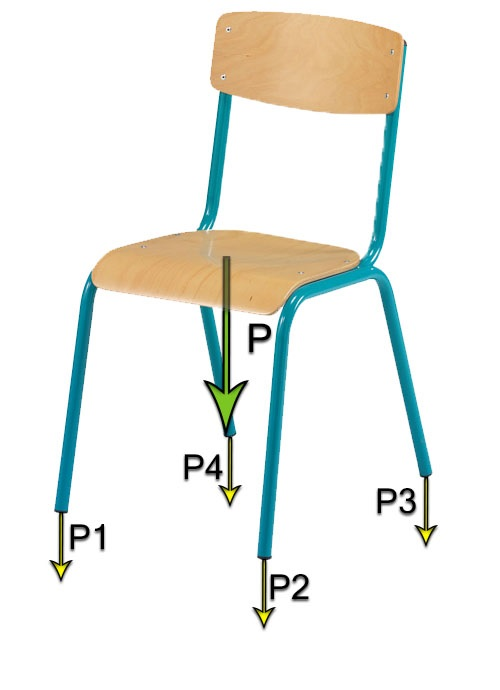
\includegraphics[scale=1]{image/Chaise_forces_homo.jpg}
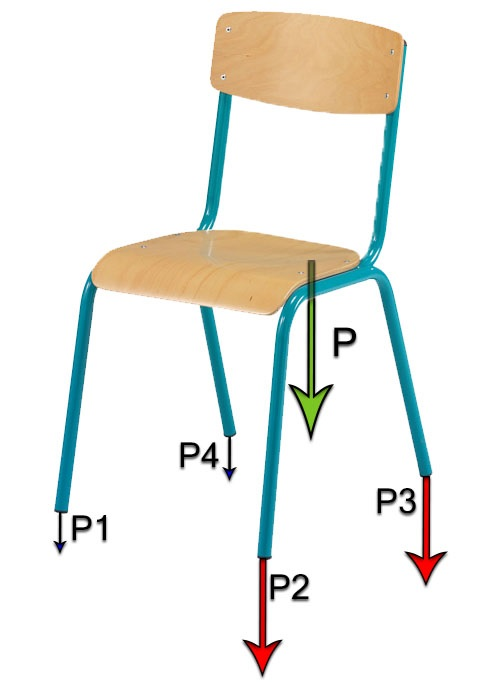
\includegraphics[scale=1]{image/Chaise_forces_hetero.jpg}
\end{center}
\caption{Illustration de la projection de la résultante des forces appliqués à la chaise vue au niveau des pieds de celle-ci pour deux position assises différentes}
\label{fig:illustr_chaise_forces}
\end{figure}

En pratique, on ne connais pas l'emplacement du point d'application de la force sur le plateau de la chaise. Or c'est déterminer sa position qui permet de définir la qualité de l'assise. Une bonne assise donnera une répartition des masses donnée et donc une position de la force totale donnée. Par exemple dans la figure \ref{fig:illustr_chaise_forces}, l'image de gauche correspond à quelqu'un qui serait assis bien droit au centre de la chaise tandis que l'image de droite correspond à quelqu'un assis (ou penché) du coté gauche de la chaise.

Cependant, connaissant la position de chaque pieds, et connaissant la valeur de la force appliquée à chaque pied, on peut trouver la position du barycentre des forces (c'est à dire, la position de la force totale et donc celle du centre de masse). 

Nous allons voir comment résoudre ce problème. Nous rappelons que le but est de déterminer la position du centre de masse, caractéristique de la posture.

Ici on considère le poids (c'est à dire les forces liés à la masse). Le barycentre des forces obtenus correspond donc au centre de masse. 
Par la suite, nos calculs se feront en 2 dimensions dans le plan du sol. En effet, on assimile les pieds de la chaise à des points du plan. On place un point $O$ origine du repère dans le plan. 

Pour chaque pieds de la chaise on associe les grandeurs suivantes:

\begin{enumerate}
\item un numéro $i$
\item un point du plan $A_i=(x,y)$ avec $x,y$ ses coordonnées
\item une valeur de force notée $m_i$ (par analogie à la masse)
\item un vecteur position $\vec{OA_i}$ représentant la position du point par rapport au point $O$
\end{enumerate}

L'idée ici est de représenter la chaise dans le plan du sol. La figure \ref{fig:schem_plan_sol_math} illustre une chaise carrée dont les quatre pieds sont projetés dans le plan du sol.


\begin{figure}[htbp]
\begin{center}
\begin{tikzpicture}
\coordinate (O) at (0,0);
\coordinate (A1) at (1,1);
\coordinate (A3) at (1,4);
\coordinate (A2) at (4,1);
\coordinate (A4) at (4,4);
\coordinate (X) at (5,0);
\coordinate (Y) at (0,5);

\draw[->] (-1,0) -- (X);
\draw (X) node[right] {$x$};
\draw [->] (0,-1) -- (Y);
\draw (Y) node[above] {$y$};
\draw (O) node[below left] {$O$} node{$\bullet$};
\draw (A1) node[below] {$A_1,m_1$} node{$\bullet$};
\draw (A2) node[below] {$A_2,m_2$} node{$\bullet$};
\draw (A3) node[above] {$A_3,m_3$} node{$\bullet$};
\draw (A4) node[above] {$A_4,m_4$} node{$\bullet$};
\end{tikzpicture}
\end{center}
\caption{Représentation de la chaise dans le plan du sol}
\label{fig:schem_plan_sol_math}
\end{figure}

Alors, on peut trouver $\vec{OG}$, vecteur position du barycentre des forces, par la formule \eqref{eq:centre_gravite}  suivante:

\begin{equation}
\label{eq:centre_gravite_vectorielle}
\vec{OG} = \frac{1}{M} \sum_i m_i  \cdot \vec{OA_i} =   \frac{1}{\sum_i m_i} \sum_i m_i  \cdot \vec{OA_i} 
\end{equation}

Avec $G$ qui est le point du barycentre, $M=\sum_i m_i$ est la somme des forces associés aux pieds.

L'équation \eqref{eq:centre_gravite_vectorielle} est vectorielle c'est à dire qu'elle est valide pour les coordonnées $(x_G,y_G)$ du point $G$.

C'est à dire qu'on a les relations \eqref{eq:centre_gravite_cartesienne}.

\begin{equation}
\label{eq:centre_gravite_cartesienne}
x_G = \frac{1}{M} \sum_i m_i  \cdot x_{A_i} \Leftrightarrow  y_G = \frac{1}{M} \sum_i m_i  \cdot y_{A_i}
\end{equation}

On peut donc retrouver la position du centre de masse d'une personne assise sur une chaise rien qu'en connaissant la valeur des forces au niveau de chaque pieds. La figure \ref{fig:schem_plan_sol_math_G} illustre le résultat qu'on pourrait obtenir pour le point $G$ avec une répartition des forces hétérogènes sur les pieds de la chaise.

\begin{figure}[htbp]
\begin{center}
\begin{tikzpicture}
\coordinate (O) at (0,0);
\coordinate (A1) at (1,1);
\coordinate (A3) at (1,4);
\coordinate (A2) at (4,1);
\coordinate (A4) at (4,4);
\coordinate (X) at (5,0);
\coordinate (Y) at (0,5);
\coordinate (G) at (1.7,3.3);
\coordinate (xG) at (1.7,0);
\coordinate (yG) at (0,3.3);

\draw[->] (-1,0) -- (X);
\draw (X) node[right] {$x$};
\draw [->] (0,-1) -- (Y);
\draw (Y) node[above] {$y$};
\draw (O) node[below left] {$O$} node{$\bullet$};
\draw (A1) node[below] {$A_1,m_1$} node{$\bullet$};
\draw (A2) node[below] {$A_2,m_2$} node{$\bullet$};
\draw (A3) node[above] {$A_3,m_3$} node{$\bullet$};
\draw (A4) node[above] {$A_4,m_4$} node{$\bullet$};

\draw [-] [dashed] (G) -- (xG);
\draw [-] [dashed] (G) -- (yG);

\draw (xG) node[below] {$x_G$} node{$.$};
\draw (yG) node[left] {$y_G$} node{$.$};

\draw (G) node[above right] {$G,M$} node[blue]{$\bullet$};
\end{tikzpicture}
\end{center}
\caption{Exemple de la position du centre de masse $G$ avec les valeurs de forces $m_i$ réparties de façon hétérogène sur les points $A_i$ }
\label{fig:schem_plan_sol_math_G}
\end{figure}

Nous avons donc évoqué toutes les raisons qui ont motivé le choix de mesurer des forces au niveau des pieds d'une chaise pour déterminer la position d'une personne.

L'idée, pour savoir si une personne est mal assise, est d'enregistrer la position du centre de masse lorsque la personne est bien assise. On peut ensuite comparer la position à un instant $t$ quelconque pour savoir si la personne est bien assise.

\textbf{Transition:} On sait maintenant que l'essentiel du projet consiste à acquérir la valeur des forces sous les pieds de la chaise. La partie suivante de ce rapport sera donc consacré à la réalisation de cette acquisition à l'aide de capteurs de forces et d'un Arduino.

\section{Le matériel et Arduino}
\label{chap:arduino}

Construire un correcteur de posture assise a nécessité de trouver un moyen de récupérer les informations de l'assise de l'utilisateur. Nous avons choisi de suivre la proposition de M.Beaufils qui était d'utiliser des capteurs positionnés sous les pieds d'une chaise. Ces capteurs permettent de déterminer la répartition des masses sur les 4 pieds d'une chaise et donc indirectement la qualité de l'assise de l'utilisateur. Il a été nécessaire d'utiliser un dispositif capable de mesurer les valeurs rapportées par ces capteurs. Notre choix se porte sur la proposition de M.Beaufils qui est d'utiliser un  micro-contrôleur Arduino Uno auquel sont connecté les capteurs de forces. 

Les premières séances de travail ont été consacré à des recherches sur les capteurs de forces (leurs caractéristiques et comment il fonctionnent). 

Nous avons appris pendant nos recherches que les capteurs de forces sont des résistances variables. La valeur de leur résistance varie en fonction de la force appliquée. Il existe cependant des capteurs pour lesquels la variation de résistances en fonction de la force appliquée est de l'ordre du Ohm $\Omega$ (typiquement des FSR, Force Sensitive Resistor) et d'autres pour lesquels la variation est de l'ordre du $\mu \Omega$ ou $\mathrm{m} \Omega$.

Un micro-contrôleur comme un Arduino possèdes des entrées sur lesquels il peut lire des valeurs de tensions par rapport à la masse. En effet, les pins allant de A0 à A5 sont des entrées analogiques sur lesquels on peut connecter une tension de 0 à 5V mesurable par l'Arduino. 

Avec un capteur qui se comporte comme une résistance variable, on peut confectionner un montage diviseur de tension permettant d'obtenir une tension mesurable par l'Arduino. Ce montage revient à connecter une résistance de valeur connue (on a choisit R1=10k$\Omega$) en série avec la résistance R variable du capteur et mesurer la tension aux bornes de la résistance connue.  En appliquant une tension de 5V fournie par l'Arduino au diviseur de tension, on a donc la relation suivante:

\begin{equation}
\label{eq:fsr_resistor}
U_{Capteur}= \frac{R_1}{ R + R_1} U_{Arduino} 
\end{equation}
 
 Avec $U_{Capteur}$ la tension entre la masse et le pin A0 de l'Arduino et $U_{Arduino}=5V$.
 
Au démarrage du projet nous n'avions aucune connaissance concernant les capteurs et l'Arduino. Nous avons donc expérimenté avec un capteur de force de type FSR et des potentiomètres pour simuler des capteurs dont la résistance varie selon la charge. Nous nous sommes rendu compte que le FSR est un capteur qui a une résistance presque infinie au repos et qui tend vers 0 lorsque le capteur est écrasé au maximum par une force. Nous avons alors constaté que l'Arduino peut lire des valeurs de tension entre 0V lorsqu'aucune force n'est appliquée et 5V lorsque le capteur est écrasé au maximum (d'après la formule \eqref{eq:fsr_resistor}).

Nous avons pu expérimenter avec des montages composé de 3 potentiomètres et d'un FSR connectés à l'Arduino pour faire des tests et apprendre à manipuler les données recueillies.

Nous nous sommes vite rendu compte qu'utiliser des FSR pour mesurer la répartition des masses sous les pieds d'une chaise ne serait pas adapté. En effet, le capteur sature au delà d'une pression de 2kg et nous arrivions à faire saturer le capteur avec nos doigts.

Dans un premier temps cette solution nous a convenus pendant que nous développions le microgiciel de l'Arduino et les application PC et Android que nous vous présenterons par la suite dans le chapitre \ref{chap:Application}. La figure \ref{fig:arduino_v0} présente le montage que nous avons utilisé jusqu'à la séance 6 de travail.

\begin{figure}[htbp]
\begin{center}
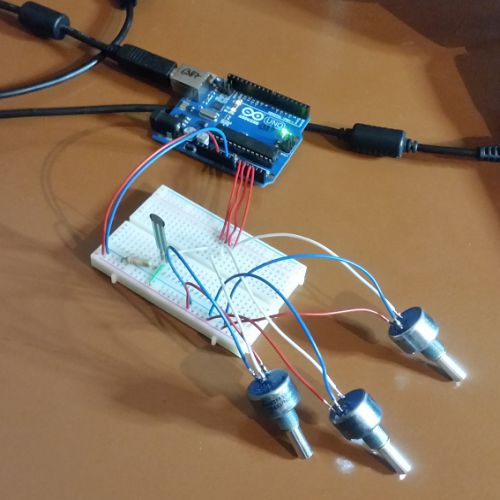
\includegraphics[scale=0.6]{image/Arduino_v0.jpg}
\end{center}
\caption{3 potentiomètres et une résistance de force connectés à un Arduino Uno}
\label{fig:arduino_v0}
\end{figure}



\chapter{Application}
\label{chap:Application}

Pour gérer les données fournies par les load sensors, nous devons construire une application qui visualise la posture assise de l'utilisateur. Pour le développement de cette application, nous avons choisi \texttt{Java} comme langage de programmation, car il est conforme avec cette tâche, et il nous est accessible à travers notre cursus académique; en réalité, tous les deux nous l'avions déjà utilisé, aussi bien pour les projets PeiP de la première année, que pour des projets personnels.

Pour mieux organiser notre workflow et afin d'avoir accès aux versions précédentes de notre logiciel, nous avons utilisé \texttt{git} comme \textit{VCS} (logiciel de contrôle des versions). Suite à la création d'un dépôt sur \texttt{GitHub}, nous avons pu synchroniser nos fichiers locaux, gérés par \texttt{git}, sur le dépôt en ligne. Cela permet de mettre en jour le projet, et \guillemotleft\ télécharger \guillemotright\ les changements qu'on y fait, avec une seule commande.

Pour que notre application soit plus fonctionnelle, nous avons décidé de mettre en place une version PC et Android. De cette manière, on permet à l'utilisateur,selon sa préférence, de consulter le correcteur de posture depuis son ordinateur ou son téléphone portable.

Le design général de l'application dans les deux cas reste le même, indépendamment de la plateforme : il y a une partie dédiée à la visualisation de la chaise, et une autre partie dédiée à la configuration (qu'elle concerne la chaise ou bien la visualisation). 

Dans la partie visualisation, le schème choisi représente tout d'abord les pieds de la chaise, symbolisés par des cercles auxquels s'associe un nombre, qui correspond au ID de chaque load sensor. Pour une chaise banale à quatre pieds, on aura donc quatre cercles, situés aux quatre coins du panel de visualisation, et portant des nombres 1, 2, 3 et 4. 

Le schèma de la visualisation comprend en outre le centre de gravité de la personne assise, qui est donné par la formule :

$$\vec{OG} = \frac{1}{M} \sum \vec{OA_i} \cdot m_i$$

où $O$ est l'origine, $G$ est le barycentre, $M$ est la somme des masses associés aux pieds, $i$ est le nombre des pieds et $A_i$ et $m_i$ sont respectivement la position et la masse du pied $i$.

Le centre de gravité est représenté par un cercle noir, qui se déplace dans le panel de visualisation suivant les changements de la posture assise de l'utilisateur.

Finalement, le schèma comprend aussi la deadzone, c'est-à-dire la zone dans laquelle la posture assise est considérée idéale. Elle est représentée par un cercle vert, dont on peut modifier la taille ainsi que la position. Cela garantit que si on a une chaise différente (par exemple une chaise à trois ou à cinq pieds), l'utilisateur peut déplacer la position de la deadzone selon ses besoins : il suffit de prendre la posture considérée comme idéale, puis de calibrer la deadzone en cliquant sur le bouton correspondant.

En somme, le schème choisi permet les manipulations suivantes :
\begin{itemize}
\item Modifier le nombre et les positions des pieds de la chaise;
\item Modifier la position et la taille de la deadzone;
\item Sauvegarder la chaise;
\item Utiliser une chaise déjà enregistrée.
\end{itemize}


Pour utiliser l'application, il faut d'abord configurer la chaise. On clique sur le bouton \guillemotleft\ configuration \guillemotright\ , on saisit le nombre des pieds de la chaise et leurs positions (on supposera que pour une chaise à quatre pieds, le pied qui se trouve devant et à gauche est au point (0,0); cela veut dire que les positions des autres pieds seront mesurées relativement au point (0,0) qu'on a défini). Une fois que la chaise est configurée, on peut se connecter à l'Arduino, soit par Bluetooth (auquel cas on doit faire un \guillemotleft\ pair \guillemotright\  afin de pouvoir se connecter), ce qui est préférable, soit par USB. Finalement, on doit s'asseoir correctement, afin de calibrer l'application. On clique alors sur \guillemotleft\ tare \guillemotright\ , puis sur \guillemotleft\ calibrer \guillemotright\  pour calibrer la position de la deadzone. Une fois qu'on l'a calibrée, la deadzone est placée dans la position considérée comme \guillemotleft\ optimale \guillemotright\ . Finalement on peut modifier sa taille selon nos préférences. 

Maintenant, l'application affichera la deadzone et le barycentre, qui deviendra rouge quand il sort de la deadzone, ce qui veut dire que notre posture n'est pas bonne. En ce point, on peut sauvegarder la chaise afin d'éviter la procédure de configuration chaque fois qu'on veut utiliser l'application. Pour ce faire, on clique sur \guillemotleft\ sauvegarder chaise \guillemotright\ , puis on choisit un dossier et un nom pour notre chaise (la chaise sera sauvegardée dans un fichier \texttt{.txt}). La prochaine fois qu'on ouvrira l'application, on pourra cliquer sur \guillemotleft\ charger une chaise \guillemotright\  et donc charger le fichier qu'on a enregistré. Ce fonctionnement nous permet aussi d'utiliser plusieurs chaises sans avoir besoin de changer la configuration chaque fois qu'on utilise une chaise différente.


%% === COMPTES RENDUS ===
\weeklyreport{11/01/2017}{Rapport seance 1}
\weeklyreport{18/01/2017}{Rapport seance 2}
\weeklyreport{25/01/2017}{Rapport seance 3}
\weeklyreport{01/02/2017}{Rapport seance 4}
\weeklyreport{08/02/2017}{Rapport seance 5}
\weeklyreport{15/02/2017}{Rapport seance 6}
\weeklyreport{08/03/2017}{Rapport seance 7}
\weeklyreport{15/03/2017}{Rapport seance 8}
\weeklyreport{22/03/2017}{Rapport seance 9}
\weeklyreport{29/03/2017}{Rapport seance 10}
\weeklyreport{05/04/2017}{Rapport seance 11}
\weeklyreport{26/04/2017}{Rapport seance 12}

\end{document}


